\chapter{Parameter Selection}
\label{ch:parameter_selection}

This chapter records the tuning parameter process and why to choose them.

\section{Random Forest}
For random forest, the parameter is to tune the trees number. The following test is based on different number. Fig~\ref{fg:rtMseDF} shows MSE, fig~\ref{fg:rtCdcDF} shows CDC, and fig~\ref{fg:rtRunTimeDF} shows running time.

\begin{figure}[h]
	\centering
	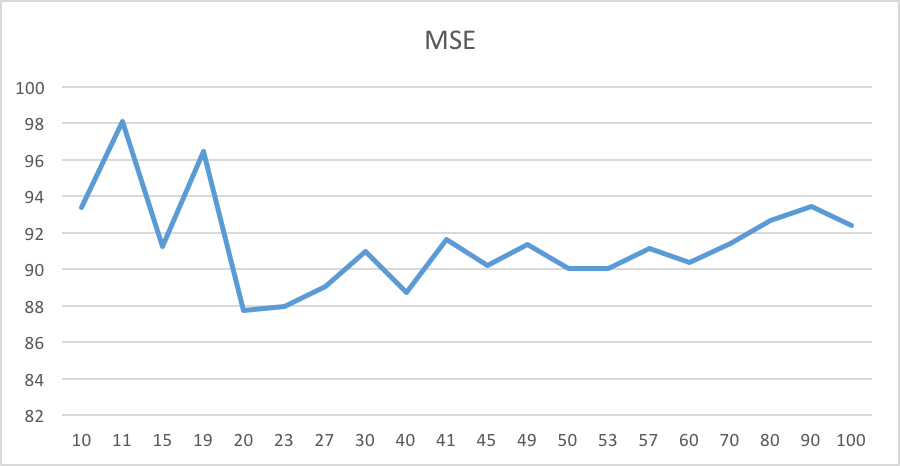
\includegraphics[width=0.8\textwidth]{FeatureSelection/rtMse}
	\caption{The average MSE result vs different random forest tree number}
	\label{fg:rtMseDF}
\end{figure}

\begin{figure}[h]
	\centering
	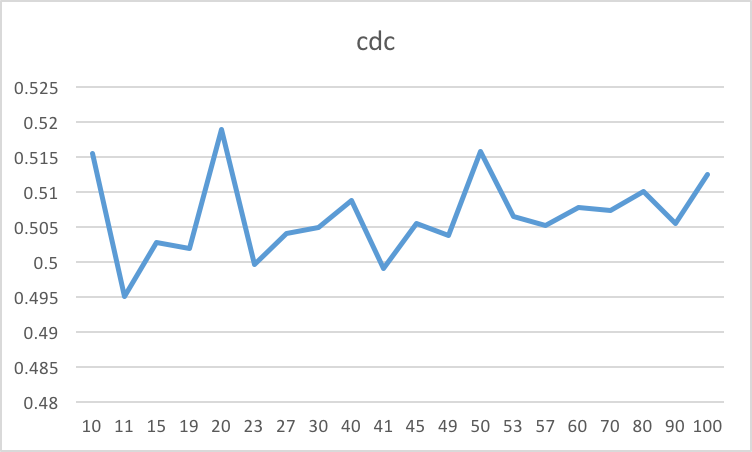
\includegraphics[width=0.8\textwidth]{FeatureSelection/rtCdc}
	\caption{The average CDC result vs different random forest tree number}
	\label{fg:rtCdcDF}
\end{figure}

\begin{figure}[h]
\centering
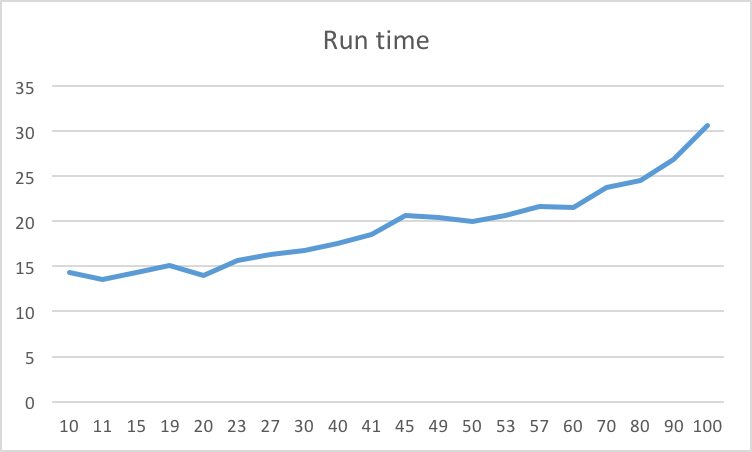
\includegraphics[width=0.8\textwidth]{FeatureSelection/rtRunTime}
\caption{The average CDC result vs different random forest tree number}
\label{fg:rtRunTimeDF}
\end{figure}

From the above figures we can find that, trees number 20 is a good point as it has almost the lowest MSE and highest CDC. As the trees number increases, the running time also increases. So in the following test, the trees number will set to 20.

\section{Artificial Neural Network}
In ANN, the number of hidden nodes is also needed to be considered. 